\section{Dimensionality reduction}

\subsection{The curse of dimensionality}

In applied mathematics, \textit{curse of dimensionality} refers to the problem caused by the exponential increase in volume associated with adding extra dimensions to a mathematical space.

Imagine we have a single measure between 0 and 1 about two types of bacteria.
\begin{figure}[H]
    \centering
    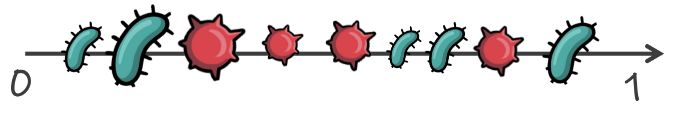
\includegraphics[width=0.3\textwidth]{images/curse-of-dimensionality-1}
\end{figure}
We would like to separate the two groups better, so we add information about another measure (i.e., \textbf{we add another dimension}). To maintain that exact same density (in our case, 9 samples per unit length) in a 2D space, we would need 81 samples.
\begin{figure}[H]
    \centering
    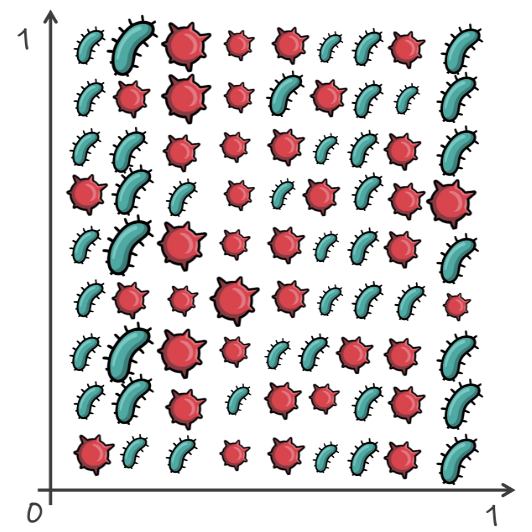
\includegraphics[width=0.3\textwidth]{images/curse-of-dimensionality-3}
\end{figure}
Because we usually only have our initial 9 samples, adding dimensions means the new space we have defined looks much wider and emptier.

At first glance, this extra space might seem like a benefit because wider space makes it easier to separate observations. In our example, the two classes of bacteria cannot be separated by a simple linear model in 2D, but adding just the third dimension does the trick.
\begin{figure}[H]
    \centering
    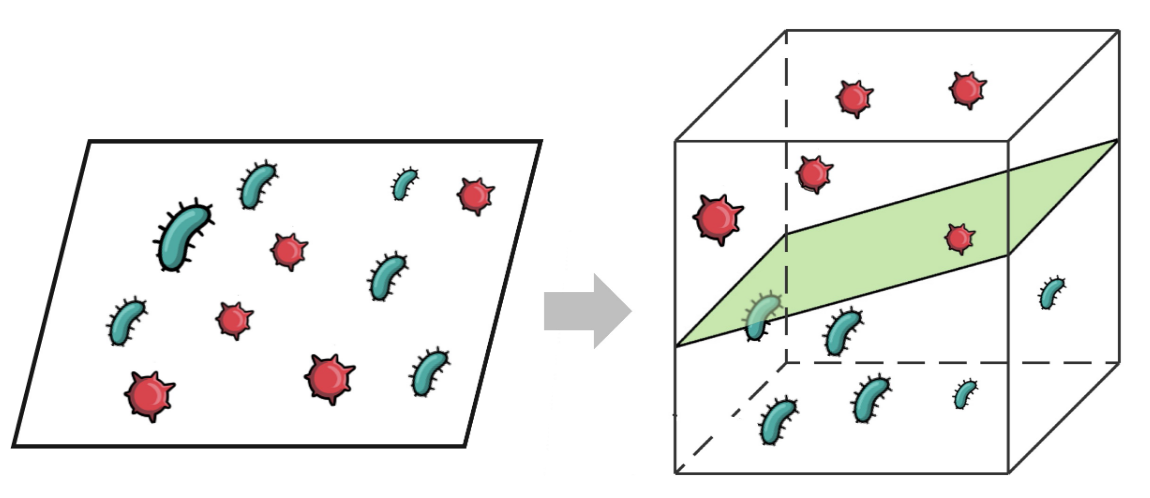
\includegraphics[width=0.5\textwidth]{images/curse-of-dimensionality-4}
\end{figure}
More dimensions give our data a higher change of being different (unique), which makes it more sparse. This introduces a higher risk of \textbf{overfitting}, meaning that whatever you learn from the data may be extremely specific to that sample.

The curse of dimensionality breaks our ability to interpret data mathematically. A fundamental rule is that \textit{n points always define a linear subspace of at most n-1 dimensions}.

When the number of predictors $p$ we measure for each data point is bigger than the number of data points ($n < p$), those predictors have to be \textbf{collinear} or \textbf{multicollinear} (the "equivalent" of linearly independent vectors). It looks like we have $p$ different predictor variables, but really some of them are linear combinations of the others, so they don't add any information. This ruins our analysis because our research objective is oftentimes to find out how each predictor is impacting the target variable individually.

Let us now consider the following linear model:
$$
y = \beta_0 + \beta_1 x_1 + \beta_2 x_2 + \varepsilon
$$
In a healthy model, the parameter $\beta_1$ represents the increase in $y$ for a unit increase in $x_1$, keeping $x_2$ and (all other covariates) fixed. But in a high-dimensional situation where multicollinearity exists, our independent variables are highly correlated: if we change $x_1$, then $x_2$ also changes, making it impossible to see their individual effect on $y$.

Lastly, another facet of the course of dimensionality is \textbf{distance concentration}. As the dimensionality of the data increases, \textit{all the pairwise distances between different points in the space converge to the same value}. This is counterintuitive: while with more dimensions the data points become more sparse (distant from each other), the gap between the minimum distance and the maximum distance between any set of points become negligible.

If every data point is practically the exact same distance away from every other point, the entire concept of proximity breaks. This avoids any algorithm that relies on measuring distance to determine similarity.

\subsection{Principal Component Analysis (PCA)}

Consider a dataset represented by a data matrix $X$ of dimensions $n \times p$, where $n$ is the number of statistical units (our observations) and $p$ is the dimension of a single unit (the features or variables we measured). Often, these $p$ variables are correlated.

Principal Component Analysis (PCA) is a dimensionality reduction technique. The primary goal of dimensionality reduction is to summarize this data containing many ($p$) variables into a smaller set of ($k$) derived variables. This will transform our original $n \times p$ matrix $X$ into a smaller $n \times k$ matrix $M$.

However, whenever we reduce dimensions, we leave behind some information from $X$ that is not retained in $M$. This lost information is called \textbf{residual variation}. We must balance the clarity of representation and ease of understanding against the risk of oversimplification (losing important information).

PCA aims at explaining the variability of the features contained in $X$ trhough a few linear combinations of these variables.

\subsubsection{Information is variability}

Variability is a fundamental concept in statistics. Imagine our statistical units are a cluster of red blood cells, and we have measured two features for each cell: its \textit{thickness} and its \textit{diameter}.

What if we wanted to simplify our dataset and describe these cells using only a single feature instead of two? If we discard thickness and only use the cell's diameter, we lose a lot of information. Cells that have vastly different thicknesses might have the same diameter, making them look much more similar than they actually are. The situation is similar if we decide to keep only the thickness instead.

Because information is directly tied to how much the data varies, our goal is to find a way to capture the maximal variability within our dataset. In our example, instead of being forced to choose between the \textit{thickness}-axis or the \textit{diameter}-axis, we can use as axis the direction along which the data points \textbf{spread} the most. This new axis is called \textbf{principal component}.
\begin{figure}[H]
    \centering
    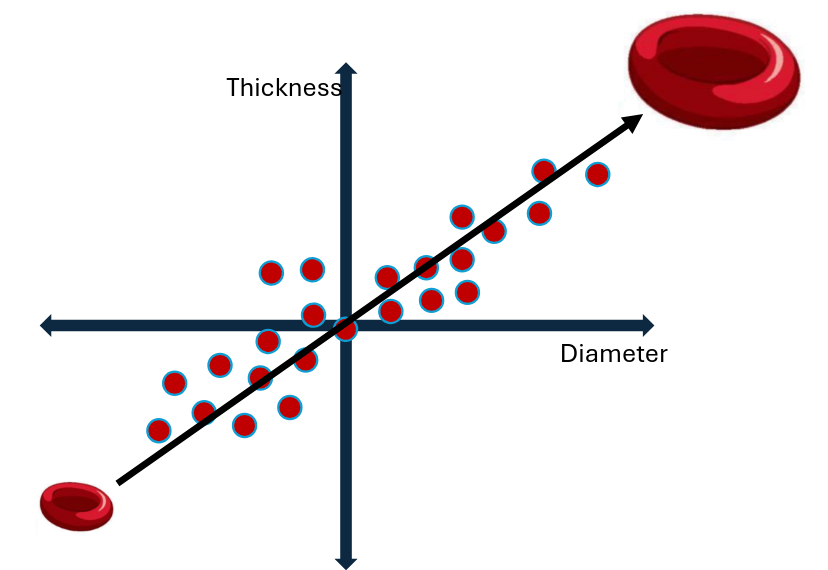
\includegraphics[width=0.4\textwidth]{images/pca-1}
\end{figure}

\subsubsection{Geometric perspective}

PCA achieves dimensionality reduction by projecting the data along these directions of maximal variability. When we draw a new line (a principal component) through our data points, our geometric goal is twofold:
\begin{enumerate}
    \item \textbf{Maximize variance}: we want the projected points (the red dots on the new line) to be as spread out as possible.
    \item \textbf{Maximize residuals}: we want the original data points (the blue dots) to be as physically close to the new line as possible.
\end{enumerate}
\begin{figure}[H]
    \centering
    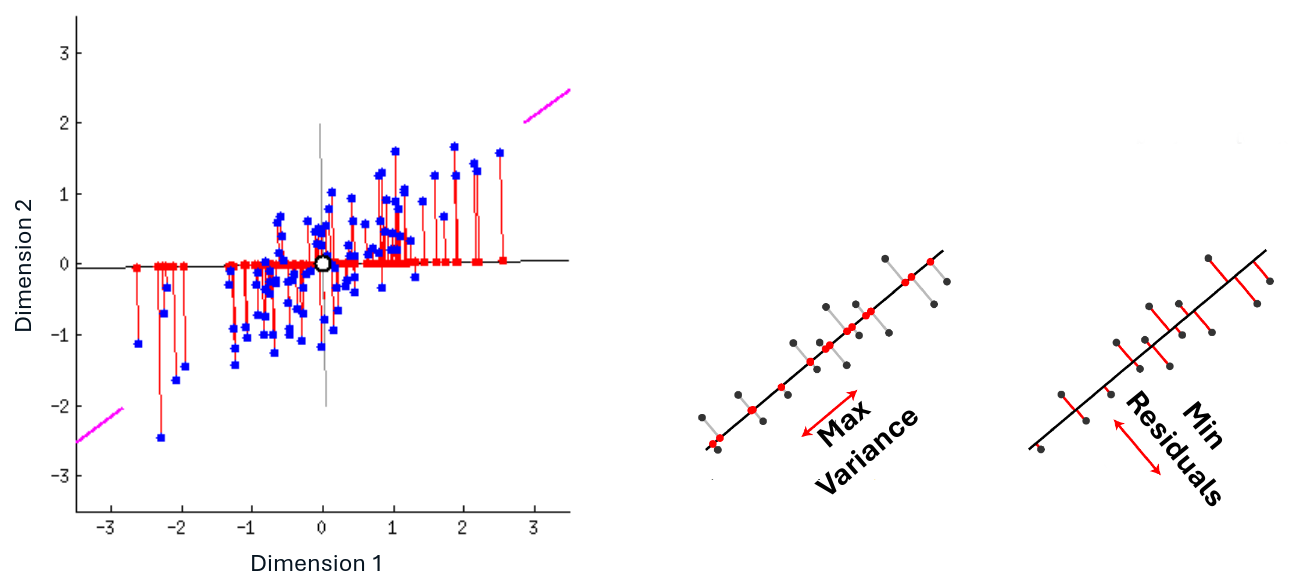
\includegraphics[width=0.8\textwidth]{images/pca-2}
\end{figure}
The result of PCA is an entirely new reference system for our cloud of points. However, before we can find this new system, we \textit{must} \textbf{center} our original data on the origin $(0,0)$ of the initial reference system. Mathematically, we achieve this by subtracting the mean vector from all points:
$$
\mathbf X_{centered} = \mathbf X - \bar{\mathbf X} = (X_1 - \bar X_1) + (X_2 - \bar X_2)
$$
Most of the times, data is also \textbf{scaled} by dividing by the standard deviation.

\subsubsection{Finding the new reference system}

Let's look at the math behind finding this new reference system. Assume we have \textit{centered} data points $x^{(1)}, \dots, x^{(n)} \in \mathbb R^p$, meaning the mean of the points is zero:
$$
\frac 1 n \sum_{i = 1}^n x^{(i)} = 0
$$
We want to choose a \textbf{direction} defined by a unit vector $u \in \mathbb R^p$ (i.e., $\lVert u \rVert_2 = 1$). If we project a data point $x^{(i)}$ onto this vector $u$, the resulting 1D score is calculated with:
$$
z_i = u^\top x^{(i)} \in \mathbb R
$$
Since our data is centered, our projected scores $z_i$ will also have a mean of 0. Therefore, the sample variance of our new scores is simply the average of the squared projections:
$$
Var(z) = \frac 1 n \sum_{i = 1}^n z_i^2 = \frac 1 n \sum_{i = 1}^n \left( u^\top x^{(i)} \right)^2
$$
So our goal is to find:
$$
\boxed{\max_{u \in \mathbb R^p} \frac 1 n \sum_{i = i}^n \left(u^\top x^{(i)} \right)^2 \quad \text{s.t.} \quad \lVert u \rVert_2 = 1}
$$
We can simplify this optimization problem using the empirical covariance matrix, denoted as $\Sigma$ and defined as:
$$
\Sigma = \frac 1 n \sum_{i = 1}^n x^{(i)} x^{(i)\top} \in \mathbb R^{p \times p}
$$
Bu substituting this into our variance equation, we get:
$$
Var(z) 
=
\frac 1 n \sum_{i = 1}^n \left( u^\top x^{(i)} \right)^2
=
u^\top \left( \frac 1 n \sum_{i = 1}^n x^{(i)} x^{(i)\top} \right) u
=
u^\top \Sigma u
$$
So the optimization problem becomes:
$$
\boxed{\max_{u \in \mathbb R^p} u^\top \Sigma u \quad \text{s.t.} \quad \lVert u \rVert_2 = 1}
$$

\subsubsection{Solving the optimization problem}
\label{sec:solving_the_optimization_problem}

To solve our constraint optimization problem, we can follow these steps:
\begin{enumerate}
    \item \textbf{Turn the constraint into an equation}:
        $$
        \lVert u \rVert_2 = 1 \iff u^\top u = 1
        $$
    \item \textbf{Build the Lagrangian $\mathcal L$}. We introduce a scalar multiplier $\lambda$, then combine our objective function and our constraint into a single equation:
        $$
        \mathcal L(u, \lambda) = u^\top \Sigma u - \lambda (u^\top u - 1)
        $$
    \item \textbf{Take the derivative with respect to $u$ and set it to zero}. To find the maximum, we use calculus. We have that for a symmetric matrix $\Sigma$:
    $$
        \nabla_u (u^\top \Sigma u) = 2 \Sigma u,
        \qquad
        \nabla_u(u^\top u) = 2u
    $$
    Applying these rules, we get:
    $$
        \nabla_u \mathcal L = 2\Sigma u - 2 \lambda u = 0
    $$
    If we divide the entire equation by 2 and rearrange it:
    $$
    \boxed{\Sigma u = \lambda u}
    $$
    In other words, any stationary point (our candidate for the optimum vector) must be an eigenvector of the covariance matrix $\Sigma$, and the multiplier $\lambda$ corresponds to its eigenvalue.
    \item \textbf{Decide which eigenvector gives the maximum}. Because our objective was to maximize $u^\top \Sigma u$, and we know that $\Sigma u = \lambda u \implies u^\top \Sigma u = \lambda$, the solution is simply the eigenvector with the largest eigenvalue. Such eigenvector is called \textbf{Principal Component 1 (PC1)}, denoted as $u_1$ with eigenvalue $\lambda_1$. We can then define $u_2$ as the eigenvector with the second-largest eigenvalue $\lambda_2$, and so on.
\end{enumerate}

\begin{figure}[H]
    \centering
    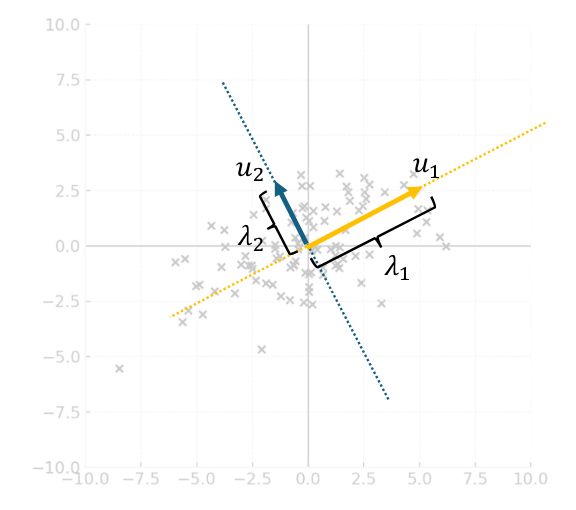
\includegraphics[width=0.4\textwidth]{images/pca-3}
\end{figure}

\subsubsection{Variance explained}

We would like to understand how much of our data's original information is actually preserved when we throw away some of the dimensions.

In PCA, information is directly equated to variance. Therefore, each principal component explains a specific proportion of the total variance within the data. If we were to keep all of our new components, between them, they would explain everything, i.e., they capture all the variability in the data. By design, PC1 always explains the most variance, PC2 explains the next highest amount, and so on.

To understand how much information a single component holds, we first need to know how much information exists in total. Assuming that all of our original variables have been centered to have zero mean, the total variance present in a dataset is simply the sum of the variances of the original variables:
$$
Var_{TOT} = \sum_{j = 1}^p Var(X_j) = \sum_{j = 1}^p \left( \frac 1 n \sum_{i = 1}^n x_{ij}^2 \right)
$$
Projecting our data onto our new principal components, we get a new set of coordinates $z$ (scores). The \textbf{variance explained} by any specific $k$-th principal component is calculated using these scores:
$$
Var_k = \frac 1 n \sum_{i = 1}^n z_{ik}^2
$$
Therefore, to find out the percentage of the variance that is explained by our new system, we look at the \textbf{proportion of variance explained}. Assuming we have $K$ components, it is defined as:
$$
Var_{exp} = \frac{Var_K = \sum_{k = 1}^K Var_k}{Var_{TOT}}
$$
From Section \ref{sec:solving_the_optimization_problem}, we have that the variance of the data along a principal component is perfectly equal to that component's eigenvalue:
$$
Var_k
=
Var(z_{\cdot k})
=
\frac 1 n \sum_{i = 1}^n z_{ik}^2
=
u_K^\top \Sigma u_k
=
u_k^\top (\lambda_k u_k)
=
\lambda_k
$$
Now, we said that the total variance is simply the sum of the variances of all the original variables ($X_1, X_2, \dots$). In the covariance matrix $\Sigma$ this individual variances sit right on the diagonal. The sum of a matrix's diagonal is called \textbf{trace} ($\mathrm{tr}$). Furthermore, we have that the trace of a matrix is always equal to the sum of all its eigenvalues. Therefore:
$$
Var_{TOT} = \sum_{j = 1}^p Var(X_j) = \mathrm{tr}(\Sigma) = \sum_{k = 1}^p \lambda_k
$$
Now that we know the variance of the individual components and the total variance, we can calculate the percentage of the variance that the $k$-th component explains:
$$
\text{Explained variance ratio of $k$-th PC} \qquad EVR_k = \frac{\lambda_k}{\sum_{m = 1}^p \lambda_m}
$$
Since we want to reduce the number of dimensions (i.e., using less principal components, $K < p$), we want to know how much total information is kept:
$$
\text{Cumulative explained variance ($K$ PCs)} \qquad \mathrm{CumEV}(K)= \frac{\sum_{k = 1}^K \lambda_k}{\sum_{m = 1}^p \lambda_m}
$$

\subsection{Non-linear dimensionality reduction}

PCA has a fundamental limitation: it is a strictly linear dimensionality reduction technique. It assumes that the data's underlying structure can be captured by drawing straight lines (hyperplanes) through the space. Real-world data is rarely that simple. In order to reduce the dimensionality of complex real data, we need to find a way to properly model structures that are highly non-linear

To understand why linear techniques fail, we must understand how high-dimensional data actually behaves. This brings us to a concept known as the \textbf{Manifolds Assumption}: \textit{"high-dimensional real data is not scattered uniformly across the ambient space. Rather, it often lies on a much lower dimensional, curved manifold."}.
\begin{figure}[H]
    \centering
    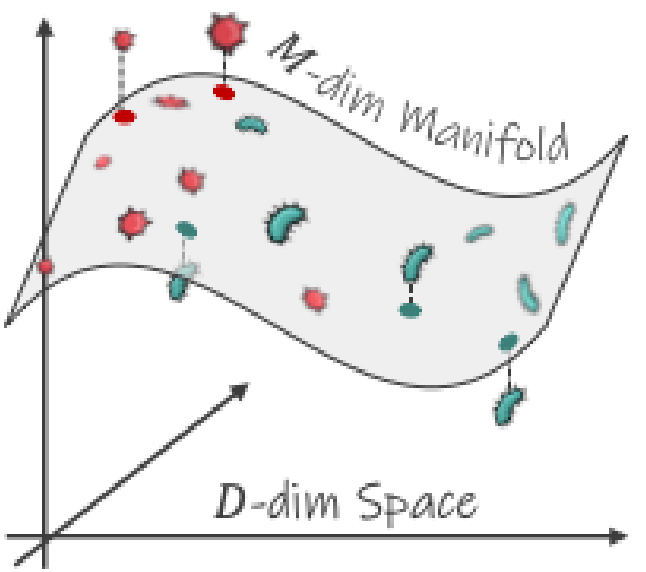
\includegraphics[width=0.3\textwidth]{images/non-linear-dimensionality-reduction-1}
\end{figure}
In other words, even if a dataset is measured with thousands of variables (a massive ambient space), the actual meaningful variation in the data is usually constrained to a much smaller, highly curved, low-dimensional manifold embedded within that space. Therefore, in order to reduce dimensionality of real data, we need to find a way to properly model the non-linear, complex shape of the manifolds that best approximates them.

To tackle these complex curved manifolds we can rely on three main philosophies, each with a different mathematical objective:
\begin{enumerate}
    \item \textbf{Linearize the structure (Kernel PCA family)}: the data might be highly non-linear in its original space $\mathbb R^D$, but if we apply a non-linear feature mapping function $\phi(x)$, the data might become "more linear" in a new, higher-dimensional space. Once it is linearized, we can then apply standard linear techniques.
    \item \textbf{Preserve geometry via local similarity (t-SME / UMAP family)}: if two data points are near each other in the original high-dimensional space $X$, they must remain near each other in the new low-dimensional space $Y$. This is particularly suitable for visualizing complex clusters of data.
    \item \textbf{Learn a non-linear mapping (Autoencoder family)}: learn an explicit non-linear function \textit{encoder} $f_\theta$, to compress the data into an embedding ($y_i = f_\theta(x_i)$), and a \textit{decoder} $g_\phi$, to reconstruct the original data ($\hat x_i = g_\phi(y_i)$). This is valuable as it provides a reusable non-linear embedding function \textit{and} a (approximate) way to go back to the original space.
\end{enumerate}
